\documentclass{beamer}

% Some common packages
\usepackage{graphicx, color}
\usepackage{alltt}
\usepackage{booktabs, calc, rotating}
\usepackage[round]{natbib}
\usepackage{multicol}
\usepackage{amsmath, amsbsy, amssymb, amsthm, graphicx}
\usepackage[english]{babel}
\usepackage{xkeyval} 
\usepackage{xfrac}
\usepackage[normalem]{ulem}
\usepackage{fancyvrb} 
\usepackage{tikz, geometry, tkz-graph, xcolor}
\usepackage[latin1]{inputenc}
\usepackage{times}
\usepackage[T1]{fontenc}

% Shortcuts
\newcommand{\empr}[1]{{\emph{\color{red}#1}}}
\newcommand{\cov}{\mathrm{cov}}
\newcommand{\pkg}[1]{{\textbf{\texttt{#1}}}}
\newcommand{\dif}{\mathrm{d}}
\newcommand{\bigbrk}{\vspace*{2in}}
\newcommand{\smallbrk}{\vspace*{.1in}}
\newcommand{\midbrk}{\vspace*{1in}}
\newcommand{\red}[1]{{\color{red}#1}}
\newcommand{\blue}[1]{{\color{blue}#1}}
\newcommand{\green}[1]{{\color{green}#1}}
\newcommand{\calc}[1]{{\fbox{\mbox{#1}}}}
\newcommand{\Var}{\mathrm{Var}}%
\newcommand{\Cov}{\mathrm{Cov}}%

\mode<presentation>
{
  \usetheme{UTD}
  \usecolortheme[RGB={200,0,0}]{structure}
  \setbeamercovered{transparent}
}

% fancy for Verbatim?
\fvset{frame=single,framesep=1mm,fontfamily=courier,fontsize=\scriptsize,numbers=left,framerule=.3mm,numbersep=1mm,commandchars=\\\{\}}


\title[Survival Analysis]{Applied Survival Analysis Using R\\ Chapter 1: Introduction}
\author[Qi Guo]{Qi Guo}
\institute[UTD]{Department of Mathematical Sciences \\ 
The University of Texas at Dallas}
\date{April, 8 2019}
	


\begin{document}

\begin{frame}
  \titlepage
\end{frame}

% Set up UTD backgroud
\setbeamercolor*{item}{fg=red}
\bgroup
\usebackgroundtemplate{
\tikz[overlay,remember picture] \node[opacity=0.05, at=(current page.center)] {
   
\includegraphics[height=\paperheight,width=\paperwidth]{UTDbg}};}


\section[Outline]{}
\begin{frame}
  \tableofcontents
\end{frame}

\section{Definition }
\begin{frame}
\frametitle{Def}
\begin{defblock}{Survival Analysis}
	Survival analysis is the study of {\color{red} survival times} and of the {\color{red} factors} that influence them.
\end{defblock}
\end{frame}

\section{Characteristics}
\begin{frame}
\frametitle{Characteristics}
Characteristics:
\begin{itemize}
	\item The response variable is a {\color{red} non-negative} discrete or continuous random variable, and represents the time for a well-defined origin to a well-defined event.
	\item A second characteristics of survival analysis, {\color{red} censoring, arise when the starting or ending events are not precisely observed}
\end{itemize}
\end{frame}


\section{Censoring}
\begin{frame}[fragile]
\frametitle{Censoring}
Examples
\begin{enumerate}	
\item \empr{right censoring} is results when the final endpoint is only known to exceed a particular value.
\item left censoring is events are known to have occurred before a certain time.
\item interval censoring is failure time is only known to have occurred within a specified interval of time.
\end{enumerate}
\end{frame}

\pagebreak

\begin{frame}[fragile]
\frametitle{Censoring}
Symbols
\begin{itemize}
\item $T^*$: the random variable representing the time to failure(exact event time)
\item $U$: the random variable representing the time to a censoring event(censoring time)
\item $T = \min(T^*, U)$: the \empr{observed} event time
\item $\delta = I(T^* <  U)$ : $\delta$ is 0 means $T$ is a censored time, 1 means  $T$ is an observed failure time

\end{itemize}
\end{frame}

\pagebreak
\begin{frame}
\frametitle{Censoring}
Types
\begin{enumerate}
	\item Type I censoring is the censoring times are pre-specified.
	\item Type II censoring occurs the experimental objects are followed until a pre-specified fraction have failed(rare in biomedical studies)
	\item \empr{Random censoring} is when each subject has a censoring time that is statistically independent of their failure time. The observed value is the minimum of the censoring and failure times; subjects whose failure time is greater than their censoring time are right-censored.
\end{enumerate}
\end{frame}

\pagebreak
\begin{frame}
\frametitle{ Random Censoring}
Cause
\begin{itemize}	
	\item In biomedical settings, one cause of random censoring is patient {\color{red}drop out}
	\begin{itemize}
	\item If the dropout occurs truly at random, and is unrelated to the disease process, such censoring may not cause any problems with bias in the analysis.
	\item If patients who are near death are more likely to drop out than other patients, serious biases may arise.
	\end{itemize}
    \item Another cause of random censoring is {\color{red}competing events}, when a patient dies of another cause first, then that patient will be censored(Chapter 9)
	\item The cause of the censoring is essential in order to avoid biased survival estimates.
\end{itemize}
\end{frame}

\section{Clinical Trials}
\begin{frame}
\frametitle{Clinical Trials}
\begin{itemize}	
	\item The most common source of random censoring is \empr{administrative censoring}, which results because some patients in a clinical trial have not yet died at the time the analysis is carried out
	\item For these patients, the survival times are only partially observed, we know that these patients survived until the end of follow-up, such times are said to be right-censored
\end{itemize}
\end{frame}

\pagebreak
\begin{frame}
\frametitle{Clinical Trials}
\begin{figure}[h!]
 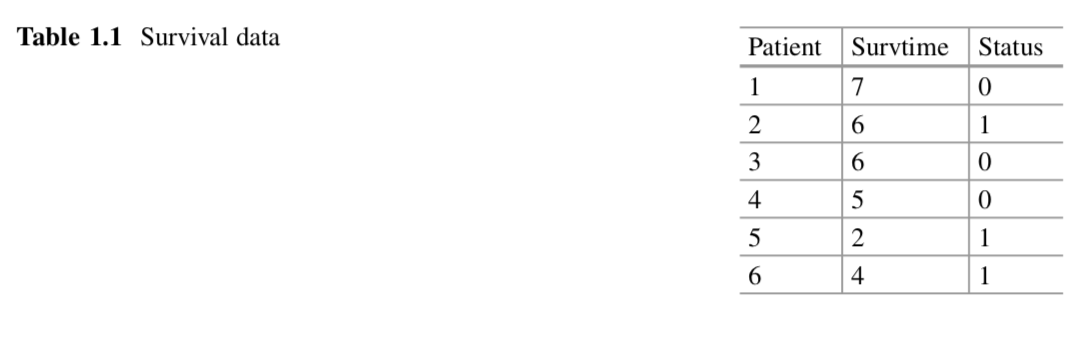
\includegraphics[scale = .35]{001.png}
\end{figure}
\begin{figure}[h!]
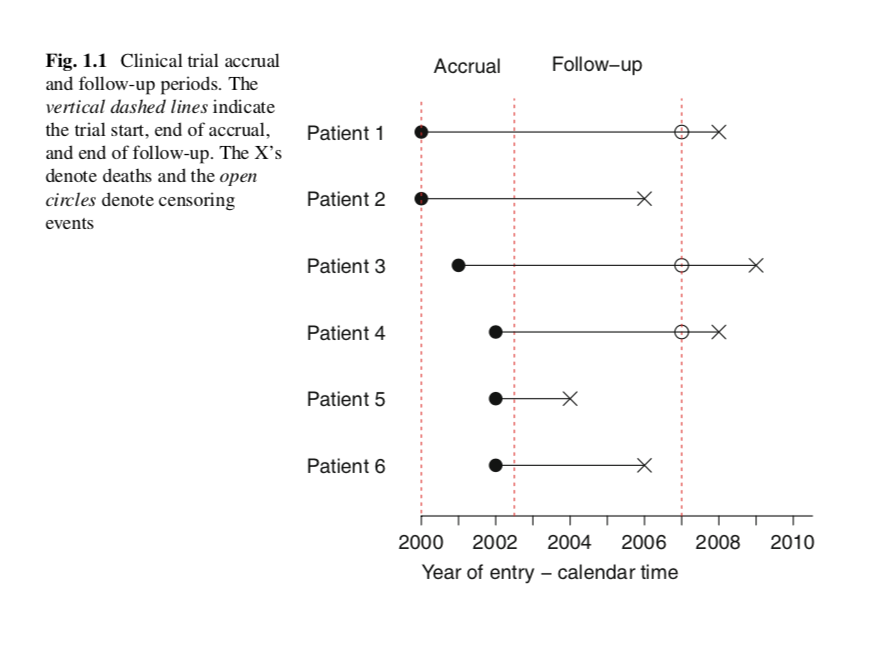
\includegraphics[scale = .35]{003.png}
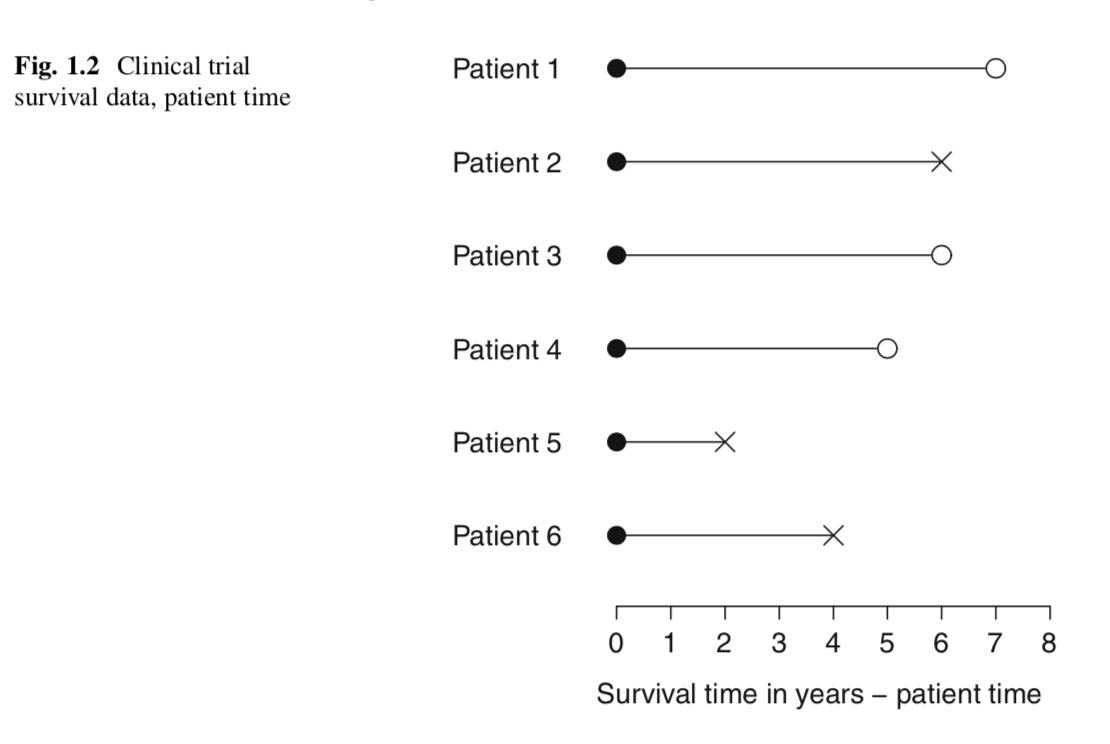
\includegraphics[scale = .3]{002.png}
 \end{figure}
\end{frame}

\section{Goal}
\begin{frame}
\frametitle{Goal}
The goals of survival analysis are to estimate the {\color{red}survival distribution}, to {\color{red}compare} two or more survival distributions, or (more generally) to {\color{red}assess the effects of a number of factors} on survival.

\end{frame}


\end{document}

